% !TeX root = ../thesis.tex

\chapter{Modell}
\label{sec:modell}
Dieses Kapitel handelt von der Herangehensweise an die praktische Umsetzung des Modells zur Vorführung seiner Funktion. In den vorausgegangenen Kapiteln wurden jegliche Grundlagen und theoretische Veranschaulichungen vertieft, welche notwendig sind um nun anwendungsorientiert in einem gegenständlichen elektrischen Sender manifestiert zu werden. Daher wurde zur Erstellung eines Modells zunächst eine \gls{acr:LT}-Spice Simulaion des analogen Signalverarbeitungsschaltkreises erstellt. Zudem beschäftigt sich dieses Kapitel mit Planung und Erstellung eines Platinenlayouts zur Komprimierung der Realisierungsgröße des Schaltkreises. Im Anschluss wird der Aufbau eines Gehäuses thematisiert, welches zur Unterbringung aller physikalischer Komponenten dienen soll.

\section{Simulation in LT-Spice}
\label{sec:simlt}

Zunächst wurde das vorausgegangene theoretische Wissen mit einer LT-Spice Simulation überprüft. So konnten eventuelle Fehler bei der Dimensionierung ermittelt und verbessert werden werden. Hierbei wurden die analogen Schaltungsteile, welche in Kapitel~\ref{sec:Signalverarbeitung} näher ausgeführt wurden zusammengefügt. Zusätzlich wurden diese durch Tiefpassfilter erweitert um hochfrequenten Störungen vorzubeugen. Ein Beispiel für ein Bauteil bei welchem ein solches Vorgehen zwingend notwendig ist, ist ein Operationsverstärker. Des weiteren wurde ein \gls{acr:DC}-Abblock-Kondensatoren zwischen Soundkarte und der ersten Stufe der analogen Signalverarbeitung vorgesehen um der Schaltung nur das reine Wechselstromsignal (\gls{acr:AC}) zuzuführen. Abbildung~\ref{fig:spice} illustriert die Simulierte Schaltung in der Darstellung des LT-Spice Softwarefensters.

\begin{figure}[H]
	\centering
	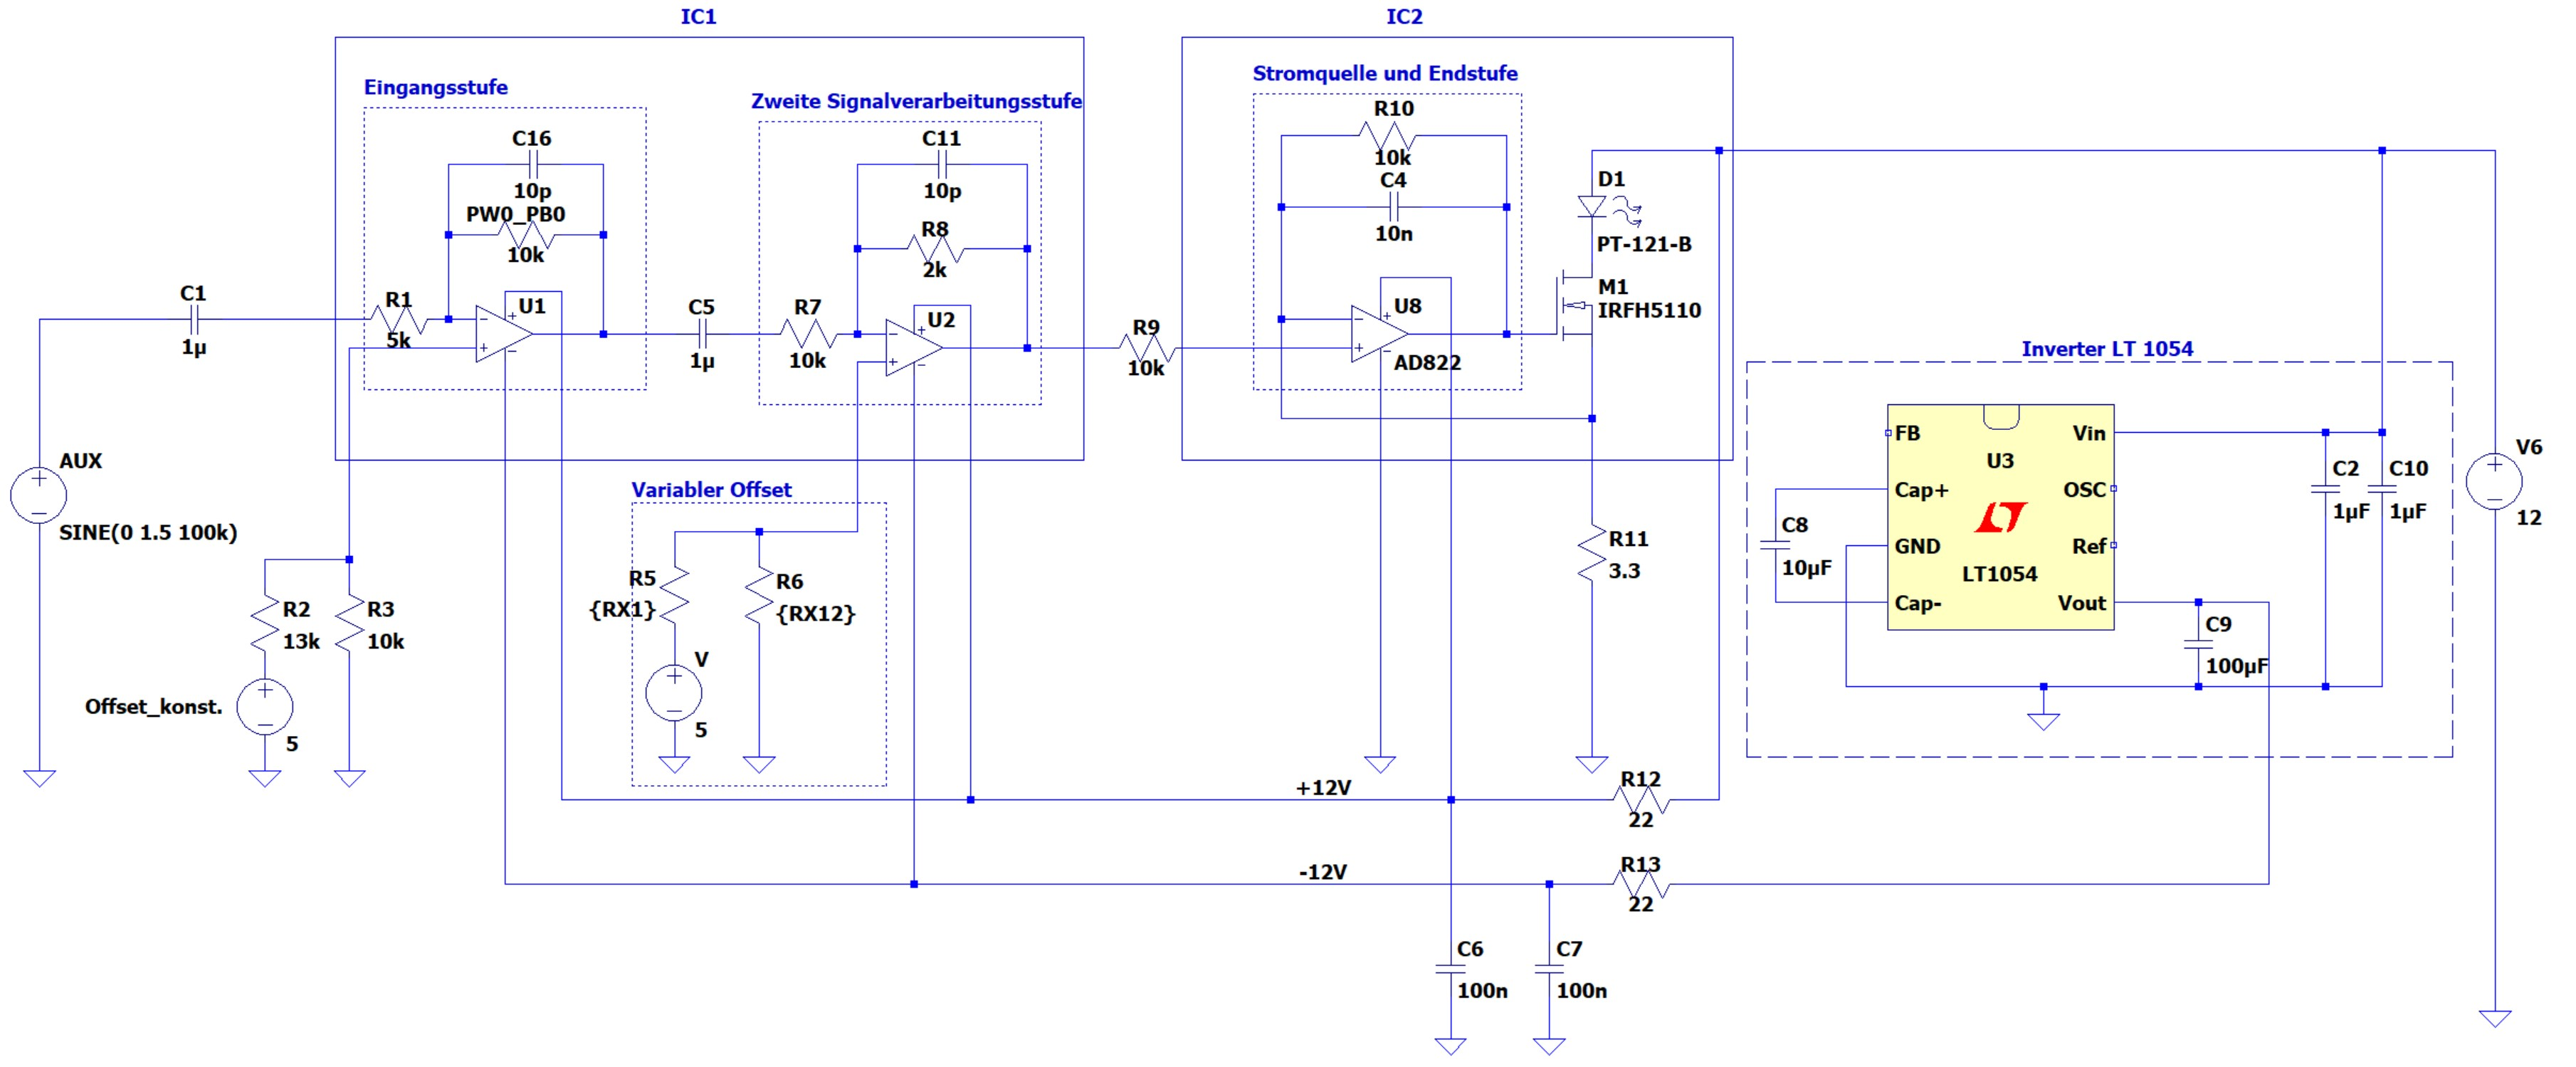
\includegraphics[width = 1 \textwidth ]{spice.jpg}
	\caption[LT-Spice Simulation der Signalverarbeitung]{LT-Spice Simulation der Signalverarbeitung} \gls{online:Eigen}
	\label{fig:spice}
\end{figure}

\section{Platinenlayout in Eagle}
\label{sec:platineeagle}

Bei dem Entwurf des Platinenlayouts für den Sender wurde ein besonderes Augenmerk auf die Trennung von Signal- und Leistungspfaden gelegt.

\begin{figure}[H]
	\centering
	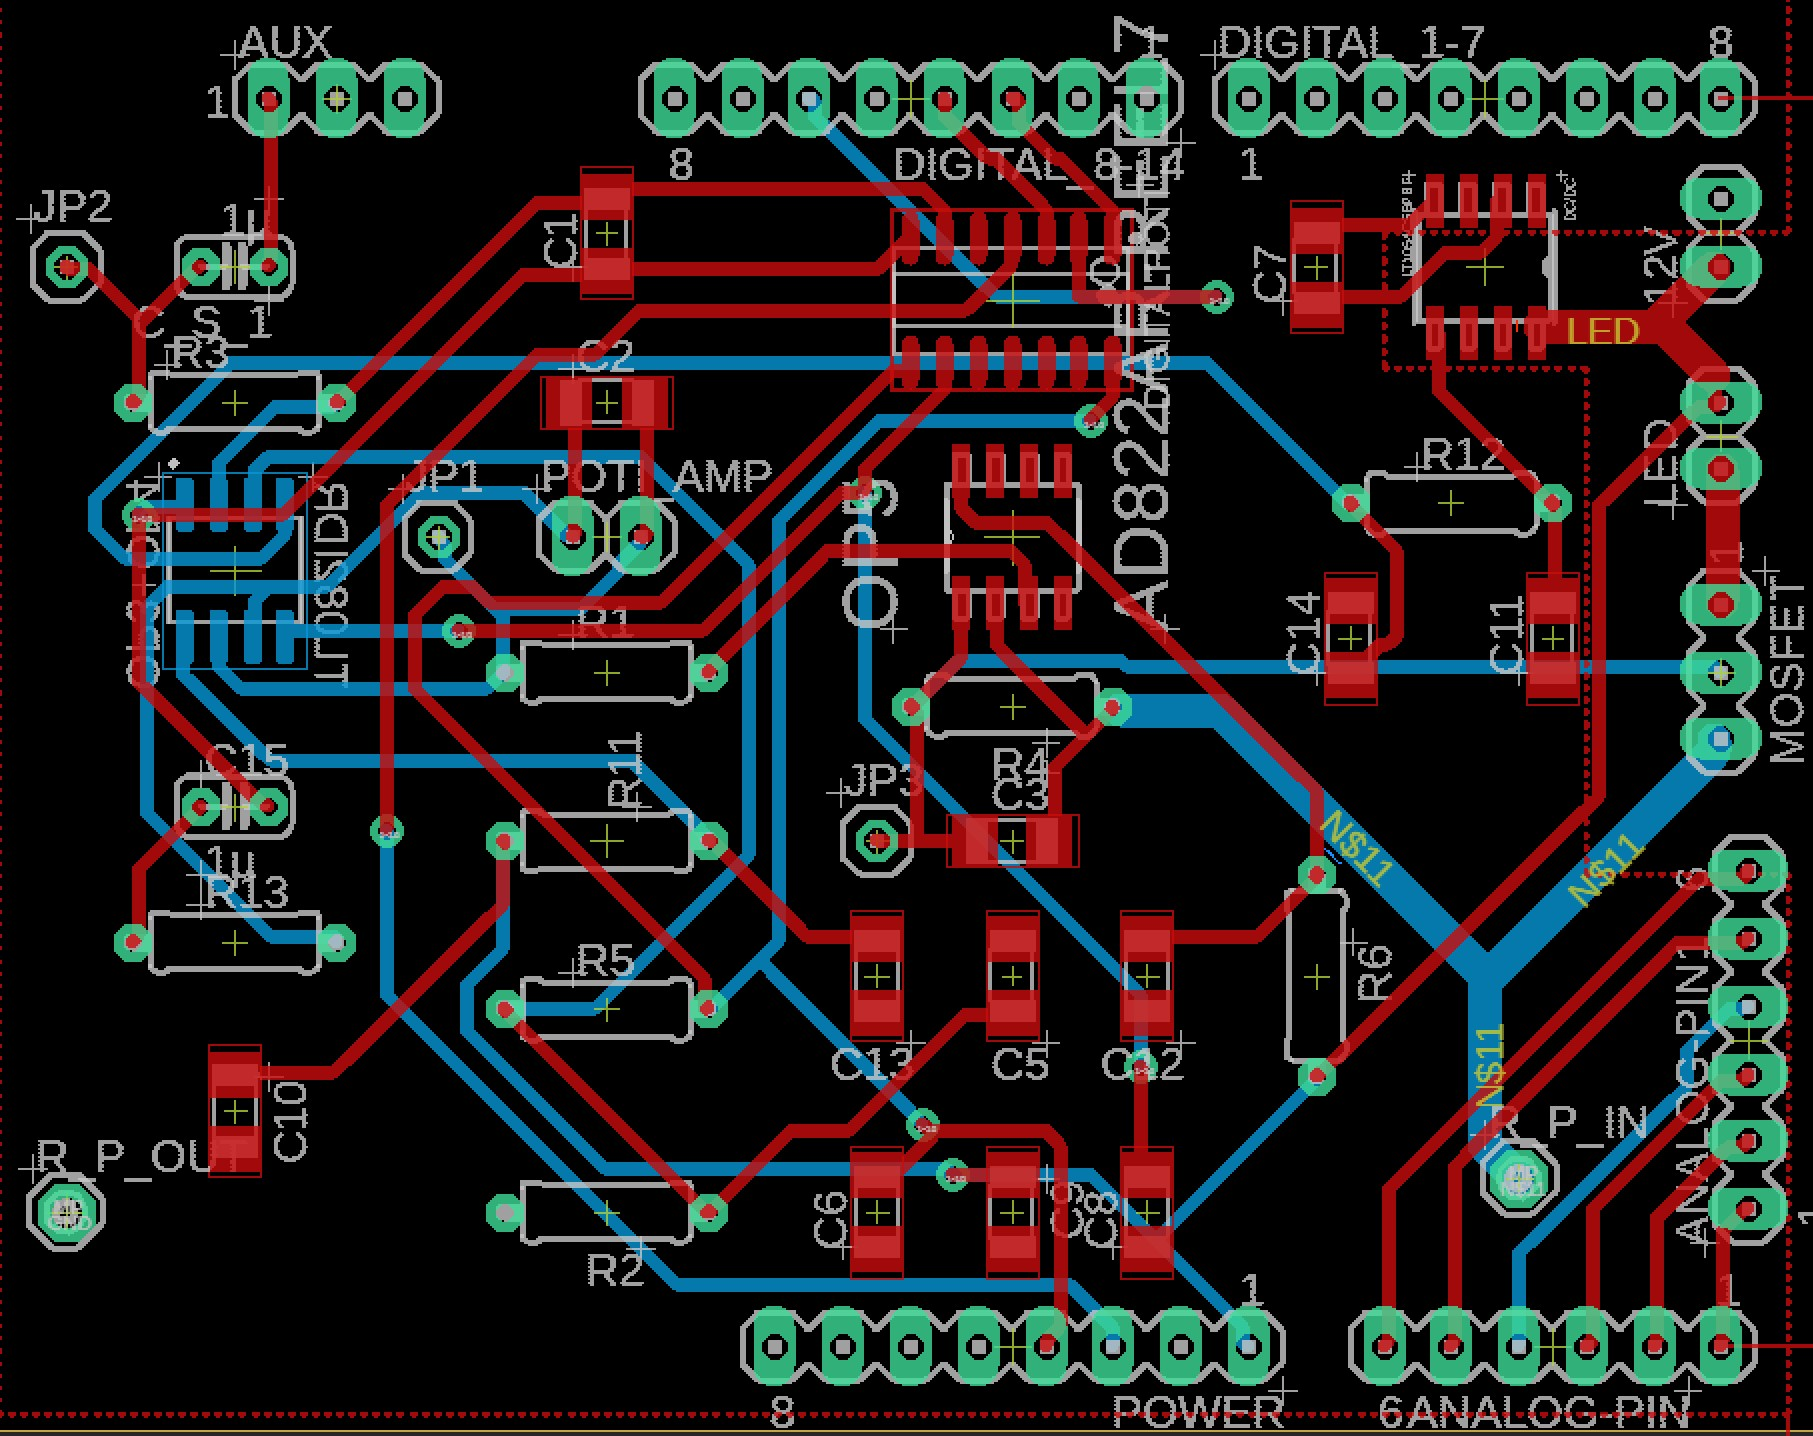
\includegraphics[width =0.8 \textwidth ]{eagle.jpg}
	\caption[Eagle Auszug der Platine]{Eagle Auszug der Platine} \gls{online:Eigen}
	\label{fig:eagle}
\end{figure}

Im unteren Bereich der Platine befindet sich der Leistungswiderstand, welcher sich von $R-P-IN$ zu $R-P-OUT$ erstreckt. Zuzüglich befinden sich der DC/DC Spannungswandler, \gls{acr:LED} und \gls{acr:MOSFET}, die signifikanten Bauteile der Stromquelle auf der rechten Seite der Platine und somit tunlichst weit vom Signalverarbeitungspfad entfernt. In der Schaltung fließen teilweise Ströme bis 1,35A. Da es bei solch hohen Strömen zu Problemen mit der \gls{acr:EMV} kommen kann, wurde der Signalweg linksseitig auf der Platine positioniert. Außerdem wurden die Leiterbahnen im Leistungspfad besonders breit ausgelegt, da hier große Ströme fließen. Genaue Informationen über die Dimensionierung der Leiterbahnen und Abstände ist in Tabelle~\ref{tab:leiterbahnen} zu finden. Diese sind signifikant für die Dimensionierung des Platinenlayouts sind Tabelle~\ref{tab:leiterbahnen}. Hier werden die verschieden Leiterbahnbreiten und Leiterbahnabstände dargestellt, welche für ein funktionierendes Platinenlayout unabdingbar sind.

\begin{table}[htb]
	\begin{center}
		\begin{tabular}[h]{cccc}	
			\toprule
			Spannung [V] & Max. Strombelastung [A]& Leiterbahnbreite [mil] & Leiterbahnabstand[mil] \\
			\midrule
			5 & 0.6&6 & 8 \\
			10 & 0.8&8 & 13 \\
			30 & 2.0&20& 30\\
			150 &2.7&30 & 50 \\
			230& 3.5&50 & 100 \\
			\bottomrule
		\end{tabular}
		\caption{Richtlinien zu Leiterbahnbreite und Leiterbahnabständen}
		\label{tab:leiterbahnen}
	\end{center}
\end{table}


Hinzu wurden auf der Platine für die Operationsverstärker, das Digitalpotentiometer und den DC/DC Spannungswandler IC-Sockel aufgelötet. Das ermöglicht den schnellen Austausch von defekten Bauteilen. Die komplette Schaltung des \gls{acr:VLC}-Senders wurde auf die Größe einer kleinen gefrästen Platine untergebracht. Deshalb wurden Leitungen auf der Rückseite der Platine verlegt. Diese sind in Abbildung~\ref{fig:eagle} durch die Blauen Leiterbahnen dargestellt. Des weiteren wurden im Signalverarbeitungspfad nach jeder Stufe Pins vorgesehen, um die Fehlersuche zu erleichtern und nachträglich einzelne Funktionsprüfungen durchzuführen. Hinzu ist zu beachten, dass die Bauteile im Leistungspfad durch den hohen Stromfluss eine hohe thermische Abgabe an Energie verzeichnen müssen. Um diese zu reduzieren wurden Kühlkörper vorgesehen. Wie diese Berechnet und Dimensioniert werden wird in Kapitel ~\ref{subsub:thermo} näher erläutert. Um die Schaltung zuletzt noch zusätzlich weniger Störanfällig zu gestalten, wurden die gegebenen freien Flächen auf beiden Seiten der Platine mit dem Masse Potential ausgefüllt. 


\section{Planung und Aufbau des Gehäuses}
\label{sec:geh}

In den vorausgegangenen Unterkapiteln wurden sowohl die Schaltungsteile, als auch die Wichtigkeit einer ausreichenden Kühlung der Bauteile verdeutlicht. Nun galt es all diese Hardwarekomponenten zu einem großen ganzen zusammen zu fassen um somit ein in sich beständiges System zu schaffen. Demnach wurde für die kompakte und ansehnliche Unterbringung aller Hardwarekomponenten ein 3D-Druck-Gehäuse projektiert. Hierbei wurde so platzsparend wie möglich gearbeitet. Aussparungen für die Datenschnittstelle und Spannungsversorgung wurden so angeordnet, dass diese jederzeit zugänglich sind. Zudem wurden drei Seiten mit ausreichend Lüftungsschlitzen bestückt, um der Wärmeentwicklung im Gehäuse entgegen zu wirken. Um diese thermische Entwicklung noch weiter unter Kontrolle zu bringen wurde eine Aussparung für einen mit $12V$ betriebenen Lüfter vorgesehen. Dieser soll den Luftstrom im Gehäuse anregen um somit eine bessere Kühlung zu gewährleisten. Abbildung~\ref{fig:3dbottom} veranschaulicht die 3D-Ansicht dieses Gehäuses.

\begin{figure}[H]
	\centering
	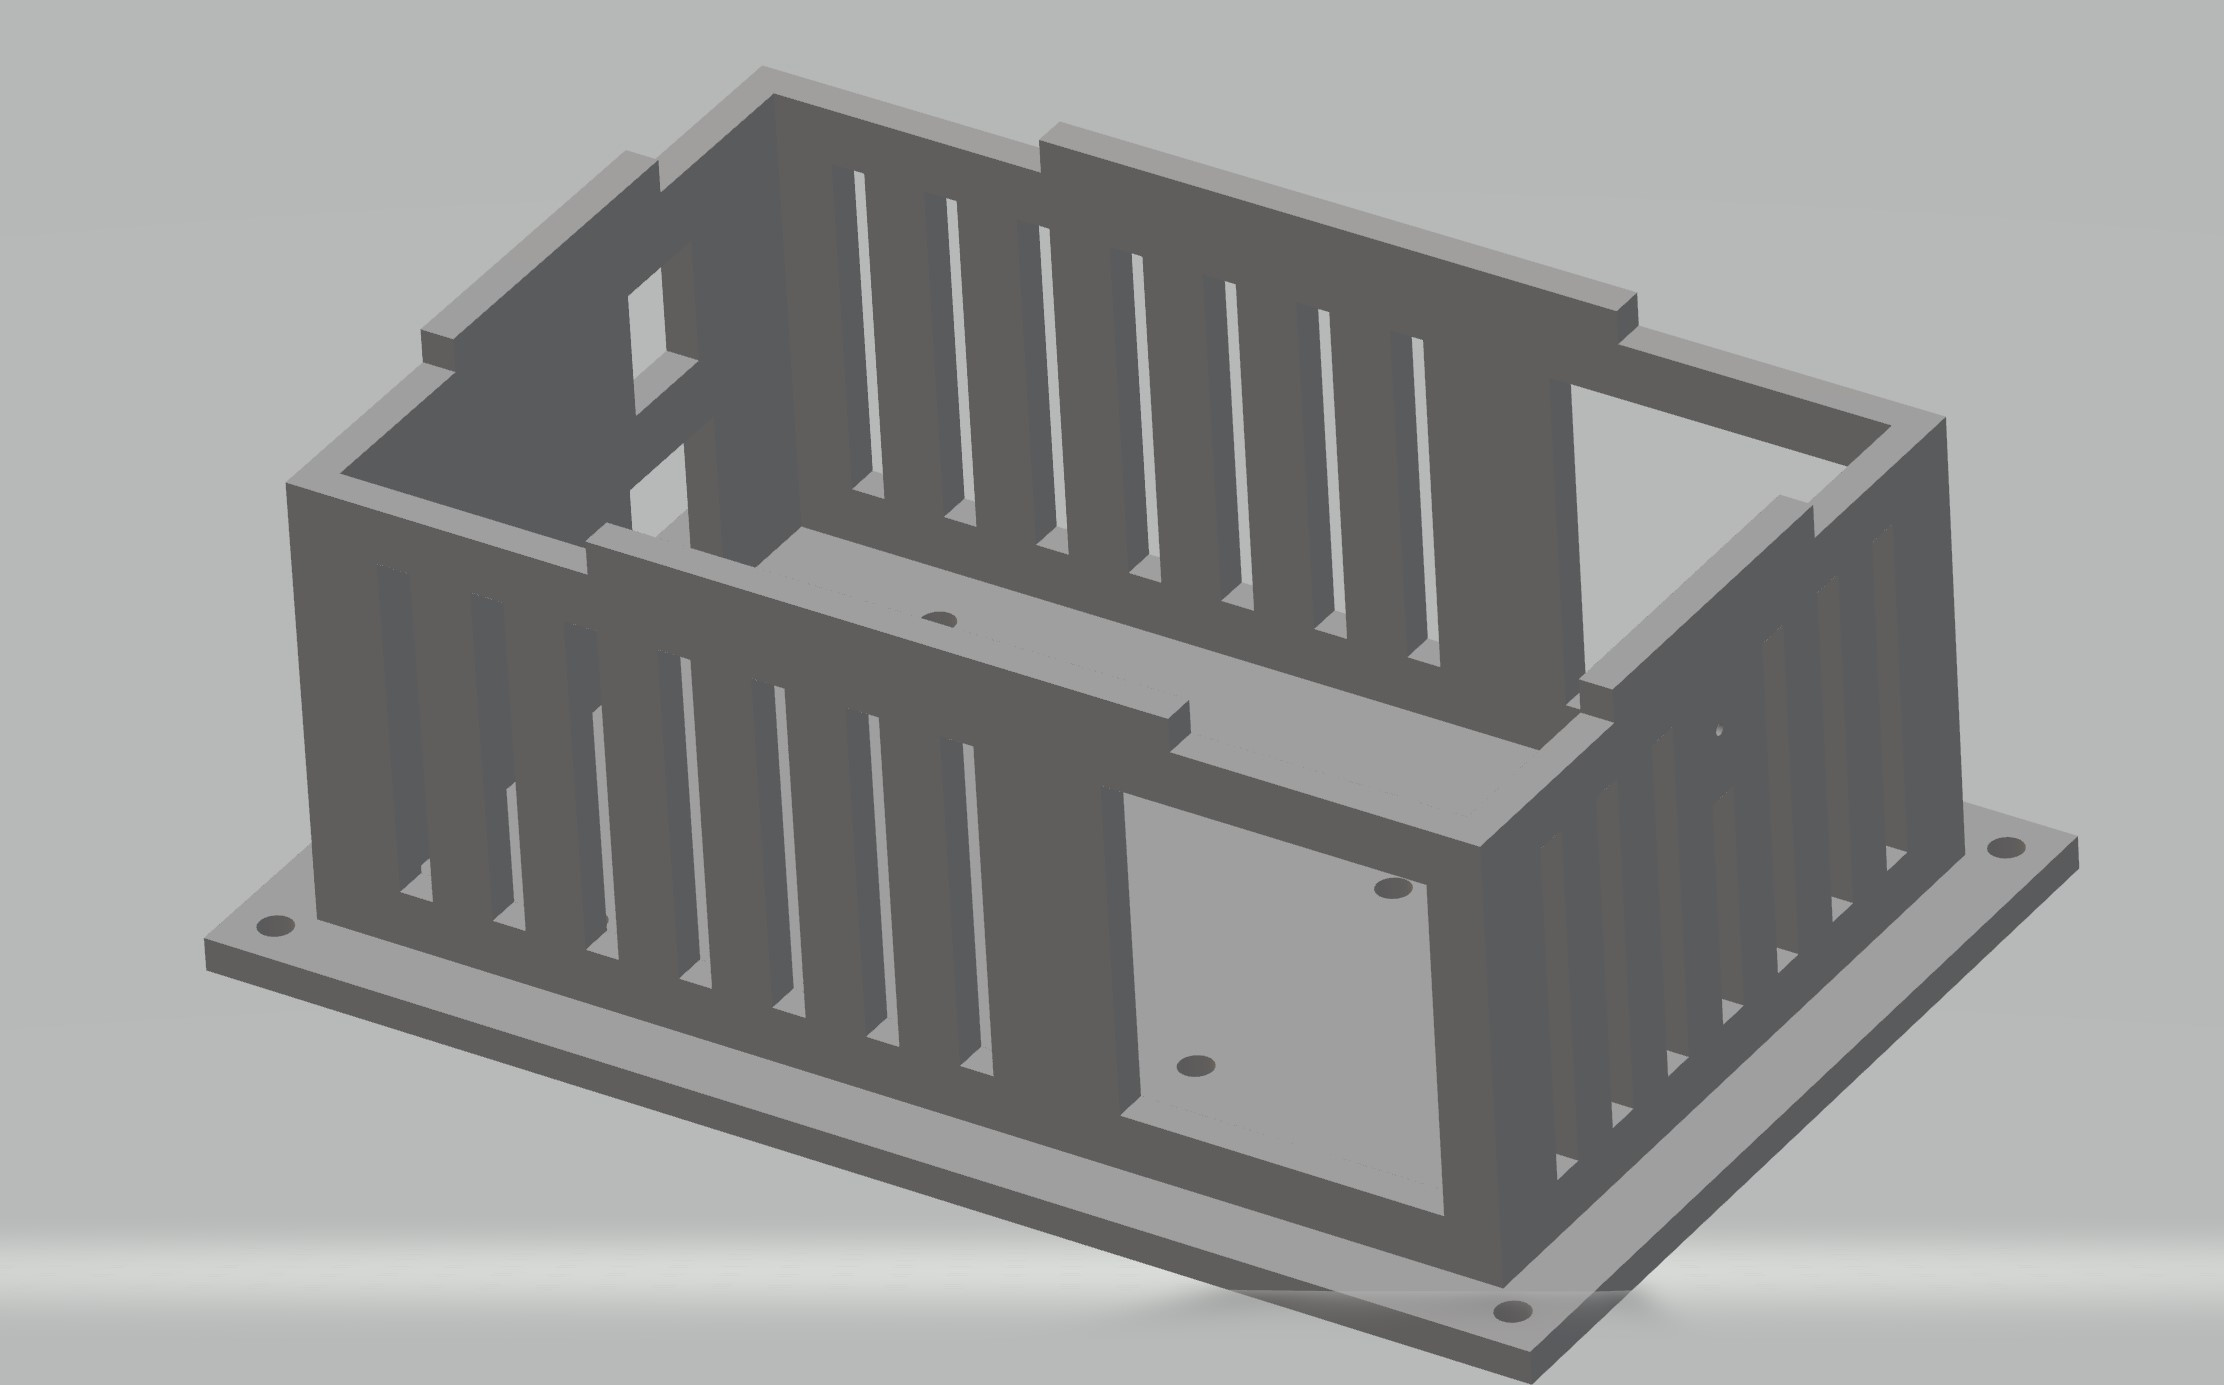
\includegraphics[width =1 \textwidth ]{3dbottom.jpg}
	\caption[Boden des 3D-Drucks]{Boden des 3D-Drucks} \gls{online:Eigen}
	\label{fig:3dbottom}
\end{figure}

Der Arduino wird am Boden des Gehäuses fixiert und bietet die Basis des Analogen Schaltungsteils.
Da sich Leistungswiderstand, Transistor und Leuchtdiode im Betrieb stark erhitzen, wurden die zugehörigen Kühlkörper nah am Lüfter montiert. Zusätzlich wurde im Deckel eine Öffnung für den Einbau eines LCD-Displays vorgesehen um dort Daten visuell am Sender auszugeben. Für die Datenübertragung wurde eine \gls{acr:AUX}-Buchse in der Nähe der Spannungsversorgung verbaut.

\begin{figure}[H]
	\centering
	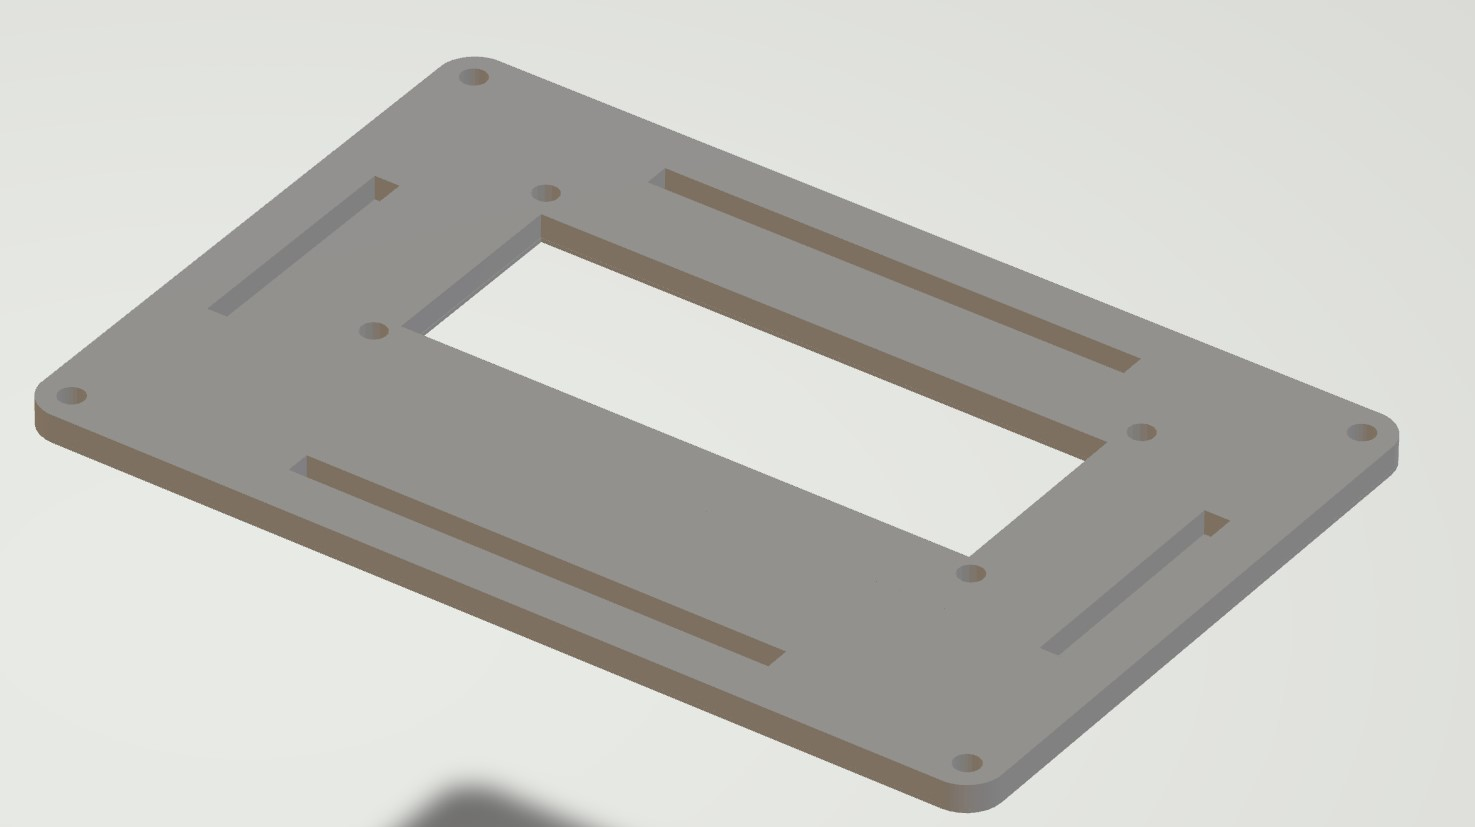
\includegraphics[width =1 \textwidth ]{3dtop.jpg}
	\caption[Boden des 3D-Drucks]{Boden des 3D-Drucks} \gls{online:Eigen}
	\label{fig:3dtop}
\end{figure}





